%\documentclass[border=5pt,tikz]{standalone}
%\usetikzlibrary{positioning}
%\begin{document}
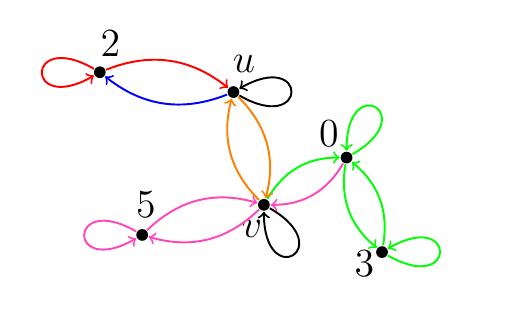
\begin{tikzpicture}[dot/.style={circle,fill,inner sep=1.5pt},line width=.7pt,x=1.5cm,y=1.5cm]
\definecolor{grenn}{rgb} {0.5,0.82,0.13}
\definecolor{pink}{rgb} {1,0.28,0.73}
\clip(0,1.3) rectangle (4,3.5);
\begin{scriptsize}
\node (r0) at (2.7,2.4) [dot] {};
\draw[color=black] (2.55,2.6) node {{\Large $0$}};

\node (r1) at (1.7420645075484014,2.9548225063123694) [dot] {};
\draw[color=black] (1.8316581320147085,3.195605372065557) node {{\Large $u$}};


\node (r2) at (0.6109449986613309,3.1228105521866865) [dot] {};
\draw[color=black] (0.7005386231276353,3.363593417939874) node {{\Large $2$}};

\node (r3) at (3,1.6) [dot] {};
\draw[color=black] (2.85,1.5) node {{\Large $3$}};

\node (r4) at (2,2) [dot] {};
\draw[color=black] (1.9,1.8) node {{\Large $v$}};

\node (r5) at (0.9693194965265414,1.7453085760172875) [dot] {};
\draw[color=black] (1,2) node {{\Large $5$}};

\draw[->,color=green] (r0) to[out=30,in=90,looseness=30] (r0);
\draw[->] (r1) to[out=-30,in=30,looseness=30] (r1);
\draw[->,color=red] (r2) to[out=150,in=210,looseness=30] (r2);
\draw[->,color=green] (r3) to[out=-30,in=30,looseness=30] (r3);
\draw[->] (r4) to[out=-30,in=-90,looseness=30] (r4);
\draw[->,color=pink] (r5) to[out=150,in=210,looseness=30] (r5);

\draw[->,color=pink] (r0) to[bend left] (r4);
\draw[->,color=green] (r4) to[bend left] (r0);

\draw[->,color=green] (r0) to[bend right] (r3);
\draw[->,color=green] (r3) to[bend right] (r0);

\draw[->,color=pink] (r5) to[bend left] (r4);
\draw[->,color=pink] (r4) to[bend left] (r5);

\draw[->,color=orange] (r1) to[bend left] (r4);
\draw[->,color=orange] (r4) to[bend left] (r1);

\draw[->,color=blue] (r1) to[bend left] (r2);
\draw[->,color=red] (r2) to[bend left] (r1);

\end{scriptsize}
\end{tikzpicture}
%\end{document}
